\documentclass[compress]{beamer}

\mode<presentation>
{
  \usetheme{Madrid}       % or try default, Darmstadt, Warsaw, ...
  \usecolortheme{default} % or try albatross, beaver, crane, ...
  \usefonttheme[onlymath]{serif}    % or try default, structurebold, ...
  \setbeamertemplate{navigation symbols}{}
  \setbeamertemplate{caption}[numbered]
  \setbeamertemplate{headline}[default]
  \setbeamertemplate{blocks}[rounded][shadow=true]
  \useoutertheme[subsection=false]{miniframes}
} 

\usepackage[utf8]{inputenc}

\usepackage[square,sort,comma,numbers]{natbib}
\usepackage{graphicx}
\usepackage{amsmath,amsthm,amssymb}
\usepackage{mathtools}
\usepackage{multicol}
\usepackage{url}
\usepackage{todonotes}
\usepackage{lipsum}

\AtBeginSection[]{\subsection{}}

\DeclarePairedDelimiter{\abs}{\lvert}{\rvert}
\DeclarePairedDelimiter{\norm}{\lVert}{\rVert}

\let\vec\mathbf
\newcommand*{\C}{%
  \mathbb{C}%
}
\newcommand*{\R}{%
  \mathbb{R}%
}
\newcommand*{\Z}{%
  \mathbb{Z}%
}

\title[Graph Kernels]{Graph Kernels and Support Vector Machines for Pattern Recognition}
\author[Léo Andéol]{\textbf{Léo Andéol}\thanks{leo.andeol@gmail.com}\\ \footnotesize Supervised by: Prof. Hichem Sahbi}
\institute[Sorbonne Uni.]{Master DAC - Sorbonne Université}
\date{May 2019}

\begin{document}

\begin{frame}
  \titlepage
\end{frame}

\section{Introduction}
\begin{frame}{Summary}
  \tableofcontents[currentsection]
\end{frame}
\begin{frame}{Motivation}

\begin{itemize}
	\item A lot of data can be represented as graphs such as proteins or social networks
	\item Being able to compare them would be useful (classification, clustering)
\end{itemize}

\begin{figure}
	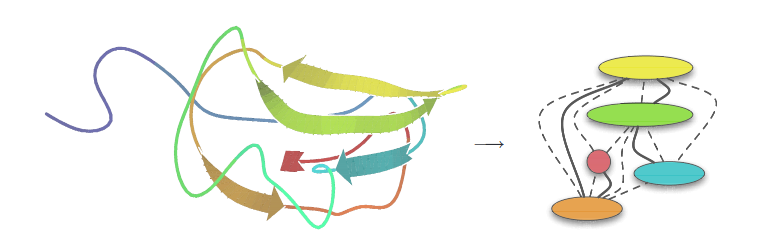
\includegraphics[width=\linewidth]{data/ecoli.png}
\caption{A fragment of a protein transformed into a graph\cite{vishwanathan_graph_2010}}
\end{figure}

\end{frame}

\begin{frame}{Current Methods}
\begin{block}{Support Vector Machine}
SVMs are models used in classification introduced about 25 years ago. They have several advantages
\begin{itemize}
	\item Great accuracy
	\item Great capacity of generalization
	\item Allows the use of kernels in its dual form
\end{itemize}
\end{block}

\begin{block}{Kernels}
	The kernel trick can replace the dot product while implicitly projecting data to a feature space and combine very well with the SVMs
\begin{itemize}
	\item Computes data projection faster implicitly (ex. RBF kernel)
	\item Improve the accuracy of SVM by making linear separation easier
\end{itemize}
\end{block}
\end{frame}

\begin{frame}{Objective}
\begin{itemize}
	\item These methods are adapted to \textbf{vector data}
	\item Graphs and their adjacency matrices aren't and vectorizing implies a loss of information
	\item New types of kernels were discovered
	\item However, the complexity is a big problem, these kernels have to be accelerated
\end{itemize}
\begin{figure}
	\begin{multicols}{2}
		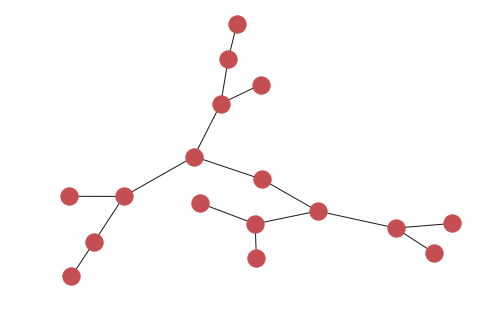
\includegraphics[width=\linewidth]{data/graphs/big_graph_no_label.png}
		$\begin{pmatrix}
		0 & 1 & 0 & 0 & 1 & 0 & 0 & 0 \\ 
		0 & 0 & 0 & 0 & 0 & 0 & 1 & 0 \\
		0 & 0 & 0 & 0 & 0 & 0 & 0 & 0 \\
		0 & 0 & 1 & 0 & 0 & 0 & 1 & 0 \\
		0 & 0 & 0 & 0 & 0 & 0 & 0 & 0 \\
		1 & 1 & 1 & 0 & 0 & 0 & 0 & 0 \\
		0 & 0 & 0 & 0 & 0 & 0 & 0 & 0 \\
		0 & 0 & 0 & 0 & 0 & 0 & 1 & 0 \\
		\end{pmatrix}$
	\end{multicols}
\caption{A tree graph and an adjacency matrix}
\end{figure}
\end{frame}


\section{Methodology}
\begin{frame}{Summary}
  \tableofcontents[currentsection]
\end{frame}
\begin{frame}{Background : graphs}
\begin{definition}
	A graph\cite{bondy1976graph} is a type of mathematical structure that represents connections between objects. It is more precisely an ordered pair $G=(V,E)$ of two sets: vertices $V$ (or nodes) and edges $E$ that connect two vertices together.
	\begin{equation*}
	E \subseteq \{(u,v) : (u,v) \in V^2\}
	\end{equation*}
\end{definition}
\begin{block}{Properties}
	\begin{multicols}{2}
		\begin{itemize}
			\item Undirected
			\item Labeled or not
			\item Degree
			\item Path and Cycle
		\end{itemize}
		\begin{itemize}
			\item Connected
			\item Tree
			\item Subgraph
			\item Line Graph
		\end{itemize}
	\end{multicols}
\end{block}
\end{frame}
\begin{frame}{Background : support vector machines}
	SVM
\end{frame}
\begin{frame}{Background : kernels}
	\begin{definition}
		In its dual form, the SVM problem only requires a dot product between the observations' vectors. 
		\begin{equation*}
		\text{max} \sum\limits_{i=1}^{n} \alpha_i - \frac{1}{2} 
		\end{equation*}
		This means the vectors can be mapped to higher dimensions with a function $\phi$. Moreover, even the dot product itself can be replaced by a function $\kappa$ without explicitly specifying the map $\phi$ as long as the function is positive semi definite.
		\begin{equation*}
		\kappa(\vec{x_{i}},\vec{x_{j}})={e}^{-\frac{\norm{\vec{x_{i}}-\vec{x_{j}}}^{2}}{2\sigma^{2}}}
		\end{equation*}
		\centering
		An example of kernel : the RBF kernel
	\end{definition}
\end{frame}
\begin{frame}{Graph Kernels}
    
\end{frame}
\begin{frame}{Graphlets}
    
\end{frame}
\begin{frame}{Random Walks}
\begin{block}{Random Walks}
	A random walk is a path obtained from a chosen vertex, randomly picking an edge to follow iteratively, until the trail reaches a certain length.
	Comparing common random walks between graphs is an acceptable metric.
\end{block}
\begin{block}{Product graph}
It has been shown\cite{imrich2000product} that computing random walks on two separate graphs is equivalent to computing it on the product graph of the two. The product graph is computed using the Kronecker (or tensor) product $\otimes$
\end{block}
\begin{figure}
\begin{multicols}{3}
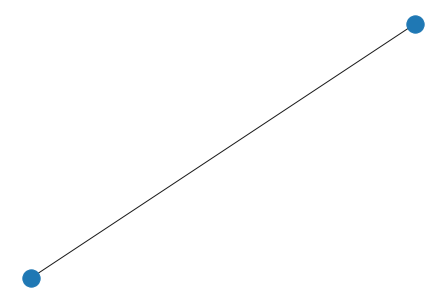
\includegraphics[width=1.5cm]{data/prod_graph/g1.png}
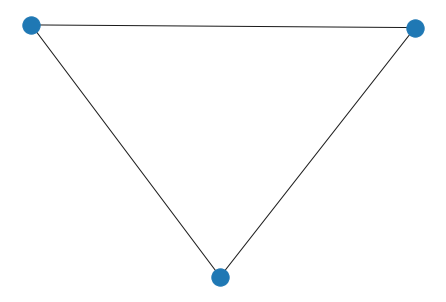
\includegraphics[width=1.5cm]{data/prod_graph/g2.png}
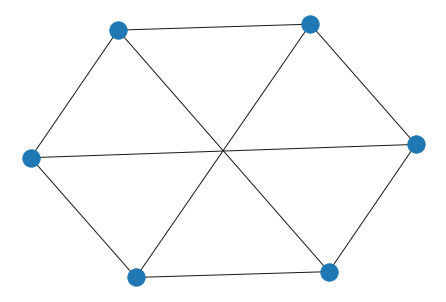
\includegraphics[width=1.5cm]{data/prod_graph/gx.png}
\end{multicols}
\caption{A graph $G_1$, a graph $G_2$ and the product graph $G_1 \otimes G_2$}
\end{figure}
\end{frame}
\begin{frame}{Random Walk}
	\begin{definition}
		kernel def
	\end{definition}
\end{frame}
\begin{frame}{Acceleration methods}
Cas particulier
\begin{block}{Inverse Kernel}
	inv ker 
\end{block}
On va vouloir accelerer machin
ce kernel va être l'objectif de plusieurs méthodes
\end{frame}
\begin{frame}{Sylvester Equation}
	content...
\end{frame}
\begin{frame}{Conjugate Gradient}
	content...
\end{frame}
\begin{frame}{Fixed Point}
content...
\end{frame}
\begin{frame}{Spectral Decomposition}
content...
\end{frame}
\begin{frame}{Nearest Kronecker Product Approximation}
\begin{itemize}
	\item The idea is to approximate two matrices $S$ and $T$ such that $\norm{W_\times - A\otimes B}_F$ is minimized.
	\item Labeled-graph kernel computation can be turned into into an unlabeled one with some loss in accuracy, but gain in computation time.
	\item Computed in $O(dn^2)$ time 
	\item All methods such as Spectral Decomposition can then be applied
\end{itemize}
\end{frame}


\section{Experiments}
\begin{frame}{Summary}
  \tableofcontents[currentsection]
\end{frame}
\begin{frame}{Frame}
    
\end{frame}

\section{Conclusion}
\begin{frame}[plain]{Conclusion}
conclu
\end{frame}

\renewcommand\bibsection{\subsection{\refname}}
\begin{frame}[plain]{References}
\nocite{bondy1976graph,borgwardt_protein_2005,imrich2000product,burges_tutorial_1998,vapnik_statistical_1998,nesterov_lectures_2018,shervashidze_efficient_2009}
\bibliographystyle{ieeetr}
\footnotesize
\bibliography{references}
\end{frame}

\appendix
\section[]{Appendix}
\begin{frame}[plain]{??}
??
\end{frame}


\end{document}